\documentclass{uvamsc}%
% \documentclass[draft]{dutmsc}%
%
% STARTING FROM VERSION 1.0.8, DIRECT PDF OUTPUT FROM THE LATEX SOURCE IS SUPPORTED.
% IF YOU WANT TO USE THIS FEATURE, MAKE SURE ALL YOUR OWN FIGURES ARE IN A FORMAT
% SUPPORTED BY PDFLATEX, SO no EPS FILES, BUT PDF OR JPEG OR SO.
% THIS HAS CONSEQUENCES FOR THE PACKAGES USED AS WELL, pstricks CANNOT BE USED WITH PDFLATEX
%
\usepackage{datetime}
% fill the following with relevant information
\mscDepartment{Computational Science}%
\mscFaculty{Informatics Institute}%
\mscName{Anand Kumar Singh}%
\newdate{date}{16}{08}{2018}
\mscDate{\displaydate{date}}%
\mscTitle{Pondering in Artificial Neural Networks}%
\mscSubTitle{Inducing systematic compositionality in RNNs}% can be left empty
\mscKeyWords{attentive guidance, sub-regular languages, pondering}%
%
% background picture for the first page, make sure it is in the correct format (eps or something else)
%\ifpdf
%  \mscBackPicture{./figs/merlin_landing_3_pdf}    % eps of 21 * 29.7 cm
%\else
%  \mscBackPicture{./figs/merlin_landing_3}    % pdf version of the cover background
%\fi
%
% readers page (un)comment as necessary
%\mscReaderOne{prof.dr. Rene Pecnik}
%\mscReaderTwo{ir.  Simone Silvestri}
%\mscReaderthree{}
%%\mscreadertwo{}
%\mscreaderfour{}
% \mscReaderFive{ir. Reader Five}
% \mscReaderSix{ir. Reader Six}
%
% if defined here with a non-zero (e.g. 1) argument, an entry will be added to 
% the table of contents for the list of figures and the list of tables,
% else they will not appear in  the toc.
\loflotintoc{1}
%
% default install of latex on linux (tetex) does not include the apacite package, so using a local version
% if your latex distribution does provide it, you can uncomment the next two lines (and comment
% the two lines after that)
% \usepackage{apacite}%
% \bibliographystyle{apacite}%
% \usepackage{./local/apacite/apacite}%
%
% If you prefer references as numbers, comment the following line and uncomment the one thereafter
% \bibliographystyle{./local/apacite/apacite}%
\bibliographystyle{plain}
%
%
% use package breakurl to break url in sensible places (such as in www references)
% if it is not available in your latex distribution, use the local one
%\usepackage[preserveurlmacro]{./local/breakurl/breakurl}
\usepackage[preserveurlmacro]{breakurl}%
\usepackage{amsmath}
\usepackage{pifont}
\usepackage{tikz,siunitx}
\usepackage{caption}
\usepackage{psfrag}
\usepackage{float}
\usepackage{nomencl}
%\usepackage{wrapfig}
\usepackage{lineno,hyperref}
\usepackage{blindtext}
\captionsetup[table]{position=bottom}

%\usepackage{./local/breakurl/breakurl}%
% \usepackage{breakurl}%
%
%=================%
% custom commands %
%=================%
%
% short-hand notations for cosine, sine and tangent with calligraphic C, S and T
\newcommand{\cc}[1]{\:\mathcal{C}_{#1}}%
\newcommand{\cs}[1]{\:\mathcal{S}_{#1}}%
\newcommand{\ct}[1]{\:\mathcal{T}_{#1}}%
%
% matlab in small caps
\newcommand{\matlab}{\textsc{Matlab} }
%
\makenomenclature
%
% setup of hyperlinks in the pdf output (modify as needed)
\hypersetup{colorlinks=true,
            citecolor=darkblue,
            urlcolor=darkred,
            linkcolor=darkblue,
            menucolor=darkblue,
            anchorcolor=red,
            pagecolor=cyan,
            pdfborder={0 0 0},
            bookmarksnumbered=true,
            breaklinks=true,
            pdfauthor={\mscname},           % value of \mscName
            pdftitle={\msctitle},           % value of \mscTitle
            pdfkeywords={\msckeywords}}     % value of \mscKeywords
%
\renewcommand{\bibname}{References}
\begin{document}%

\definecolor{greyavi}{RGB}{0.5,0.5,0.5}
\definecolor{greyavi2}{RGB}{250,250,250}
\newcommand{\thinsolidline}{\raisebox{2pt}{\tikz{\draw[-,black!40!greyavi,solid,line width = 0.4pt](0,0) -- (5mm,0);}}}
\newcommand{\thindashedline}{\raisebox{2pt}{\tikz{\draw[-,black!40!greyavi,dashed,line width = 0.4pt](0,0) -- (5mm,0);}}}
\newcommand{\solidline}{\raisebox{2pt}{\tikz{\draw[-,black!40!greyavi,solid,line width = 1.2pt](0,0) -- (7mm,0);}}}
\newcommand{\dashedline}{\raisebox{2pt}{\tikz{\draw[-,black!40!greyavi,dash pattern=on 6pt off 6pt on 6pt off 6pt,line width = 1.2pt](0,0) -- (7mm,0);}}}
\newcommand{\dashdottedline}{\raisebox{2pt}{\tikz{\draw[-,black!40!greyavi,dash pattern=on 6pt off 2pt on 2pt off 2pt on 6pt off 2pt on 2pt off 2pt,line width = 1.2pt](0,0) -- (7mm,0);}}}
\newcommand{\dottedline}{\raisebox{2pt}{\tikz{\draw[-,black!40!greyavi,dotted,line width = 1.2pt](0,0) -- (7mm,0);}}}
\newcommand{\refline}{\raisebox{2pt}{\tikz{\draw[-,black!40!greyavi2,solid,line width = 1.2pt](0,0) -- (7mm,0);}}}


%============================= Front matter ========================================
\frontmatter%
    %
    \maketitle%
    %
    % Abstract/summary
    \nonumchap{Abstract}
    %
	Deep Neural Networks are the dominant architectural paradigm in the field for artificial intelligence (AI) and 


%
    \cleardoublepage%
    %
    % thank people in this file
    \nonumchap{Acknowledgements}
    %
Acknowledge


    % signature containing place, name and date
    \signature
%
    \cleardoublepage%
    % 
    % table of contents, list of figures and list of tables
    \tocloflot%
    %
    % Nomenclature
    \printnomencl%
    \cleardoublepage%
    %
    %
    
\mainmatter%
    %
    % parts are not necessary for a thesis
    %
    %\input{title}
    %Introduction Chapter
    \chapter{Introduction}
	%Motivation
	\nomenclature{RNN}{Recurrent Neural Network}
	\nomenclature{$\rho_f$}{density of particle}
	\nomenclature{$\mu_f$}{dynamic viscosity of fluid}
	\nomenclature{$\nu_f$}{kinematic viscosity of fluid}
	\nomenclature{$C_{p,f}$}{specific heat capacity of fluid}
	\nomenclature{$C_{p,p}$}{specific heat capacity of particle}
	\nomenclature{$k_f$}{thermal conductivity of fluid}
	
	\section{Motivation}
	
	Motivation
			
		
	\section{Objectives}
		%
		Objectives
	
		
	\section{Outline}
		%
		Thesis outline

				
    %Theoretical Background
    \chapter{Theoretical Background} \label{Chapter:theory}
AG, CH, IML, GDL

    % Modelling Strategies
    \chapter{Proposed Models}\label{Chapter:proposals}

The biggest criticism of deep learning is its overt dependence on voluminous data which has lead many researchers to argue that deep networks are only good at finding pattern recognition in training distribution and therefore conform to the basic tenet of statistical machine learning that train and test data should come from the same distribution. Deep neural networks therefore are still poor at zero shot generalization to test data which despite coming from the same \lq rule space {}\rq\ don't follow the exact same distribution as training data (find a good example here). Human reasoning on the other hand is governed by a rule based systematicity which leads us to learn complex concepts from small samples which leads to zero shot generalization (example ).

\cite{Liska2018} using lookup tables (section \ref{datasets:lt}) as the testbed tried to asses the ability of a RNN network (more specifically a 60 unit LSTM followed by a 10 unit sigmoid layer) to search for compositional solution to the lookup table task. Lookup tables exhibit functional nesting and therefore a model that can find a compositional solution from the search space of all possible solutions is more likely to zero shot generalize to novel compositions. The authors established that by having additional supervision on the weights of hidden state transitions, theoretically a finite-state automata (FSA) can be induced such that the recurrent layers encode the states of this automaton. This FSA can in principle solve the lookup table task upto a finite number of compositions. They further showed that this theoretical setup can achieve zero state generalization on unseen inputs on known compositions i.e. \textit{heldout inputs} (section \ref{lt:splits}).

However when trained purely on input/output mappings without this additional supervision, the authors noted that only a small percentage of networks could converge to a compositional solution (models capable of zero shot generalizing to unseen inputs on known compositions). Additional these small percentage of models also only showed a weak form of composition wherein if for instance t1, t2 are atomic tables, then a composition task t1 t2 is indexed to prompt t1t2, instead of solving in a nested fashion viz. t1(t2(.)). (Get feedback here, see if this is clear)

Motivation for AG - Lake's work as an inspiration should come here, something about learning the trace of a program.\cite{Lake2015}. BPL sequentially builds up complex characters from primitives by bayesian sampling. 

Attention (section \ref{mtv:attn}) based seq2seq models produce a \lq soft{}\rq\ alignment between the source (latent representation of the input) and the target. Furthermore seq2seq models require thousands of samples to learn this soft alignment. However in light of the aforementioned arguments presented in favor of concentrating on primitives to construct a complex \lq composition{}\rq\ I propose the concept of \textbf{A}ttentive \textbf{G}uidance (AG). AG argues that the decoder having perfect access to the encoder state(s) containing maximum information pertaining to that decoding step, would leave to improved target sequence accuracy.

\begin{figure}
	\begin{minipage}[t]{\textwidth}
		\ifpdf
		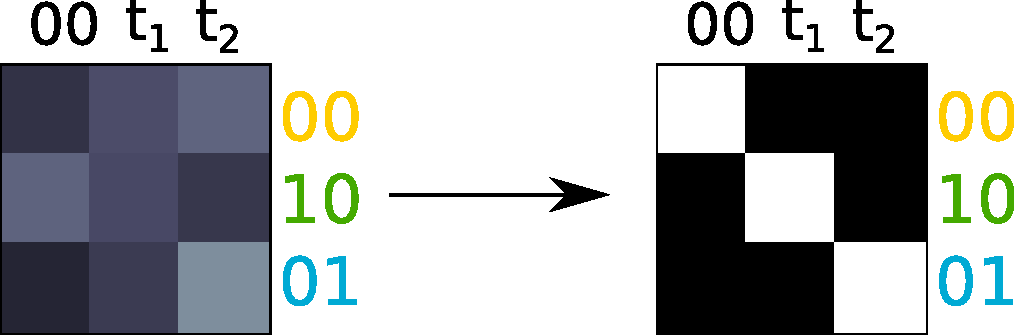
\includegraphics[width=\linewidth,keepaspectratio=true]{./figs/attention-guidance-pdf}
		\else
		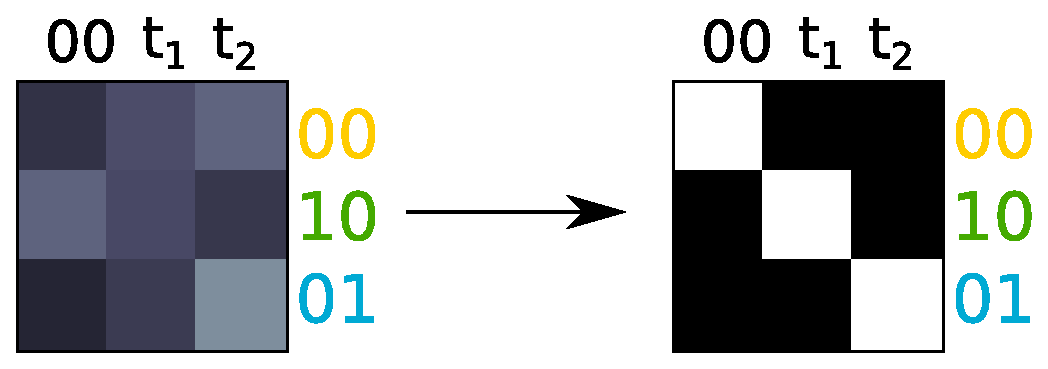
\includegraphics[width=\linewidth,keepaspectratio=true]{./figs/attention-guidance-eps}
		\fi
		\caption{\small Diffused vs Hard Attention}
		\label{pm:ag-schematic}
	\end{minipage}
\end{figure}

Revisiting the query-key-value pair view of attention described in section \ref{mtv:attn}, AG tries to improve the scalar matching score between the query and the keys during the attentive read step. Since the \textit{keys} can be thought of as the memory addresses to the \textit{values} which are needed at a given decoding step, AG tries to ensure a more efficient information retrieval. 

Write from a program learning pov as described above in Lake's work. Do mention that AG forces the model to pick the compositional solution from the space of all possible solutions. Eventually it leads to the soft alignment in standard seq2seq with attention being converted to a hard alignment. refer figure \ref{pm:ag-schematic}

\begin{figure}
	\begin{minipage}[t]{\textwidth}
		\ifpdf
		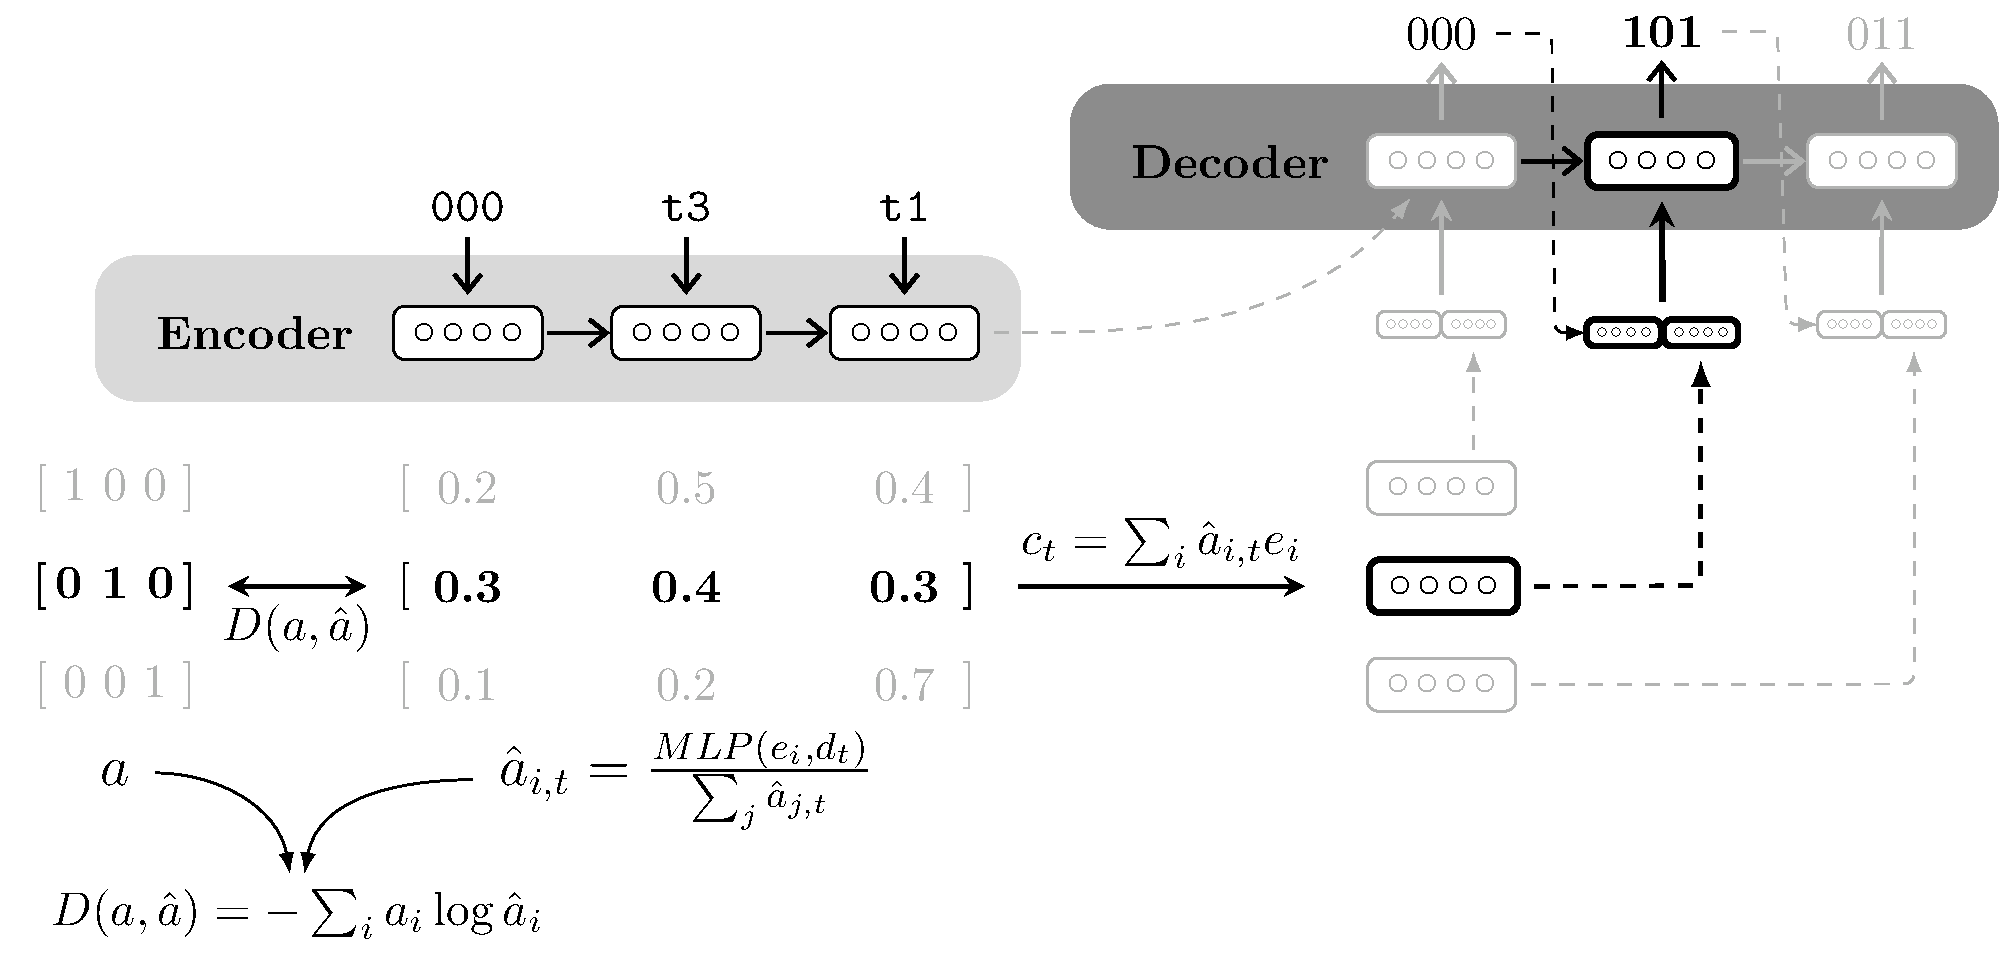
\includegraphics[width=\linewidth,keepaspectratio=true]{./figs/ag-model-pdf}
		\else
		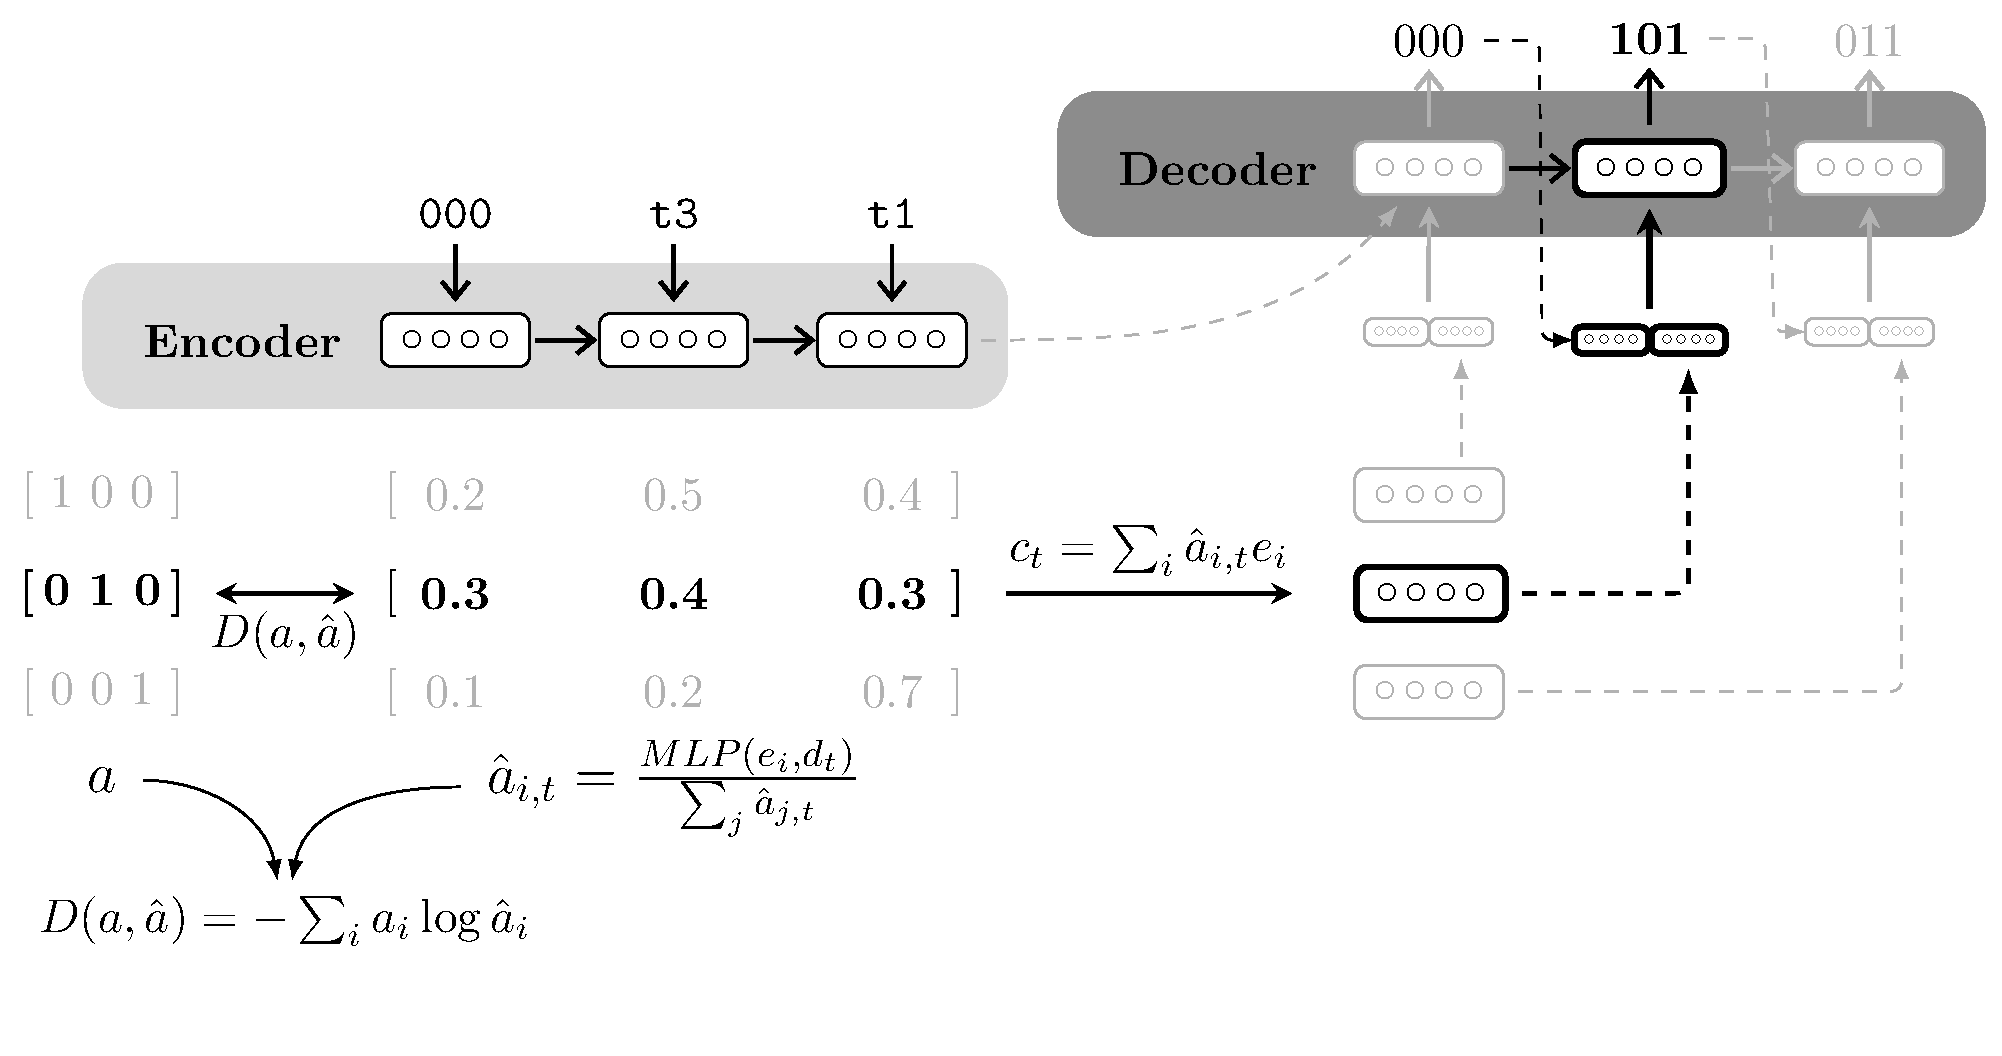
\includegraphics[width=\linewidth,keepaspectratio=true]{./figs/ag-model-eps}
		\fi
		\caption{\small Attentive Guidance and calculation of AG loss}
		\label{pm:ag-loss}
	\end{minipage}
\end{figure}

Ag is implemented via and extra loss term added to the final model loss. As shown in figure \ref{pm:ag-loss}, at each step of decoding the cross entropy loss between attention vector calculated $\alpha_{tj}$ and the ideal attention vector at that decoding step are added to the model loss. The final loss is therefore expressed as:

\begin{equation}
\widetilde{\mathcal{L}}(x,y) = \mathcal{L}(x,y) + \sum_{t=1}^T \sum_{i=1}^N -a_{i,t}\log\hat{a}_{i,t}
\end{equation}%
    %Datasets Used
    \chapter{Datasets}\label{Chapter:datasets}

\section{Lookup Tables}

\section{Symbol Rewriting}

\section{Micro Tasks}

CommAI mini tasks \citep{Baroni2017} are a set of strictly local and locally testable (please refer to section \ref{flt:sh}) languages designed to test the generalization capabilities of a compositional learner. Based on the mini tasks we propose a new dataset of sub-regular languages which we call he Micro Tasks. The language encompasses a vocabulary of all printable ascii characters, except printable but invisible characters i.e. tab, space, newline etc. 
\begin{itemize}
	\item Define verification and production tasks
	\item The vocabulary is acted upon by the boolean operators (or, and and not) in the case of both verification and production tasks. In case of verification we have an additional operation copy.
	\item Describe as in CommAI how copy and or are strictly local while and+not constitute locally k testable languages.
\end{itemize}


While the CommAI mini task position themselves as strictly local and locally testable tasks of progressive difficulty we add another layer of difficulty to the tasks by setting them up as either a decision problem(verify) or search problem(produce) in the same training domain.

\begin{figure}[ht] 
	\begin{subfigure}[b]{0.5\linewidth}
		\centering
		\ifpdf
		\includegraphics[width=0.95\linewidth]{./figs/micro/train_verify-pdf}
		\else
		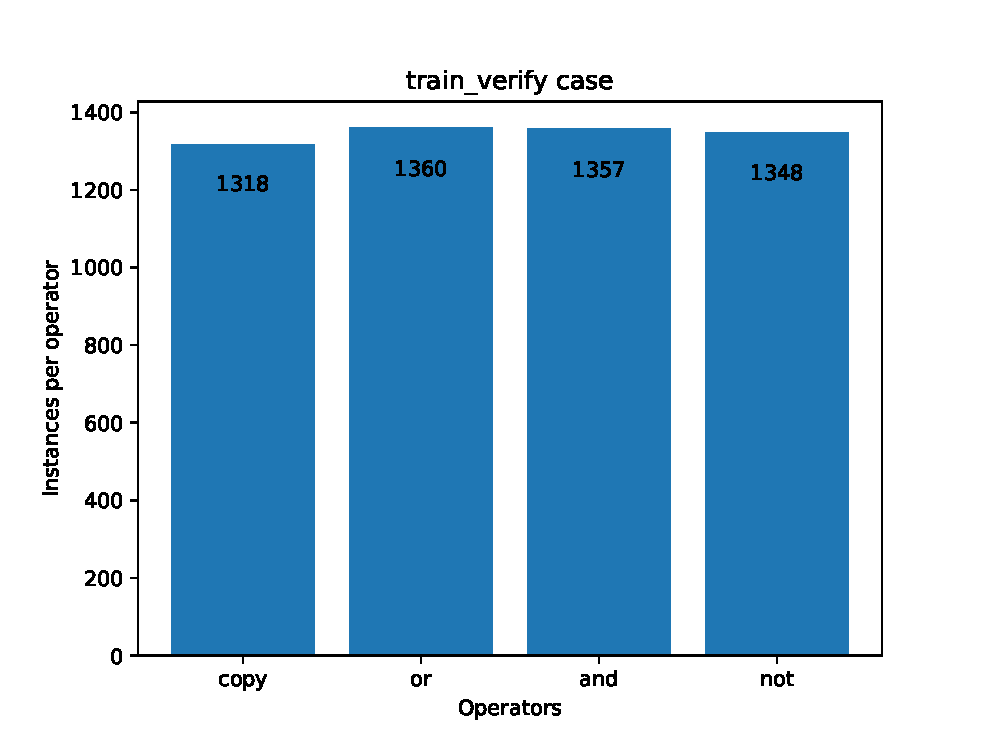
\includegraphics[width=0.95\linewidth]{./figs/micro/train_verify-eps}
		\fi
		\caption{Verification Task} 
		\label{tr_ver} 
		\vspace{4ex}
	\end{subfigure}%% 
	\begin{subfigure}[b]{0.5\linewidth}
		\centering
		\ifpdf
		\includegraphics[width=0.95\linewidth]{./figs/micro/train_produce-pdf}
		\else
		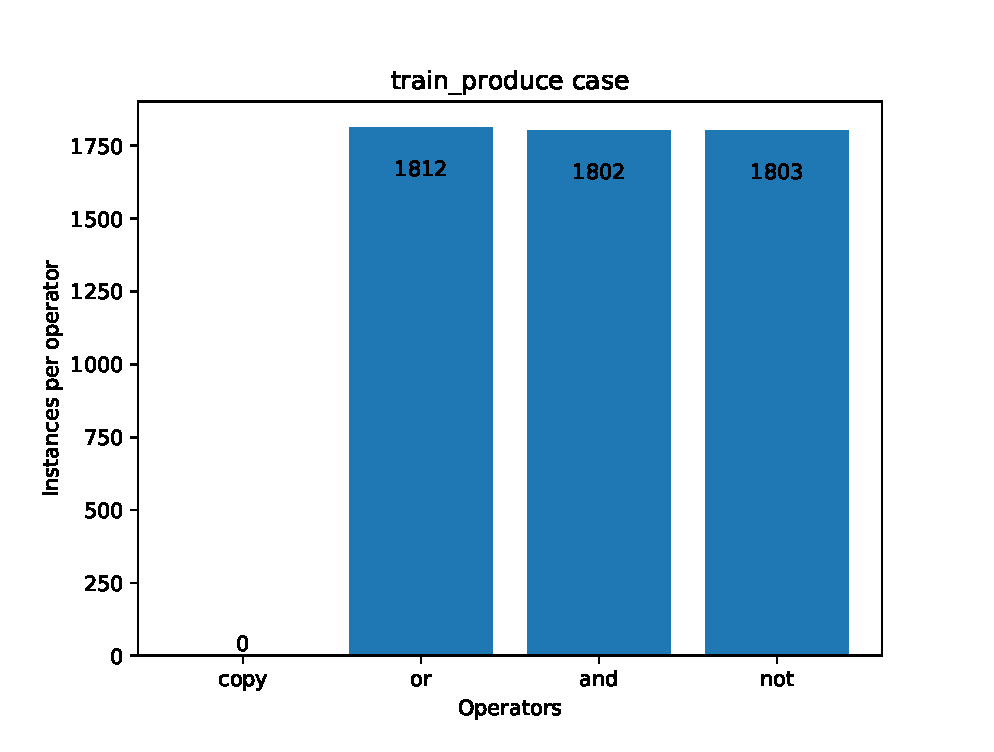
\includegraphics[width=0.95\linewidth]{./figs/micro/train_produce-eps}
		\fi 
		\caption{Production Task} 
		\label{tr_prd} 
		\vspace{4ex}
	\end{subfigure}
	\caption{Micro Tasks - Training Data}
	\label{micro_train}
\end{figure}

\begin{figure}[ht] 
	\begin{subfigure}[b]{0.5\linewidth}
		\centering
		\ifpdf
		\includegraphics[width=0.95\linewidth]{./figs/micro/unseen_verify-pdf}
		\else
		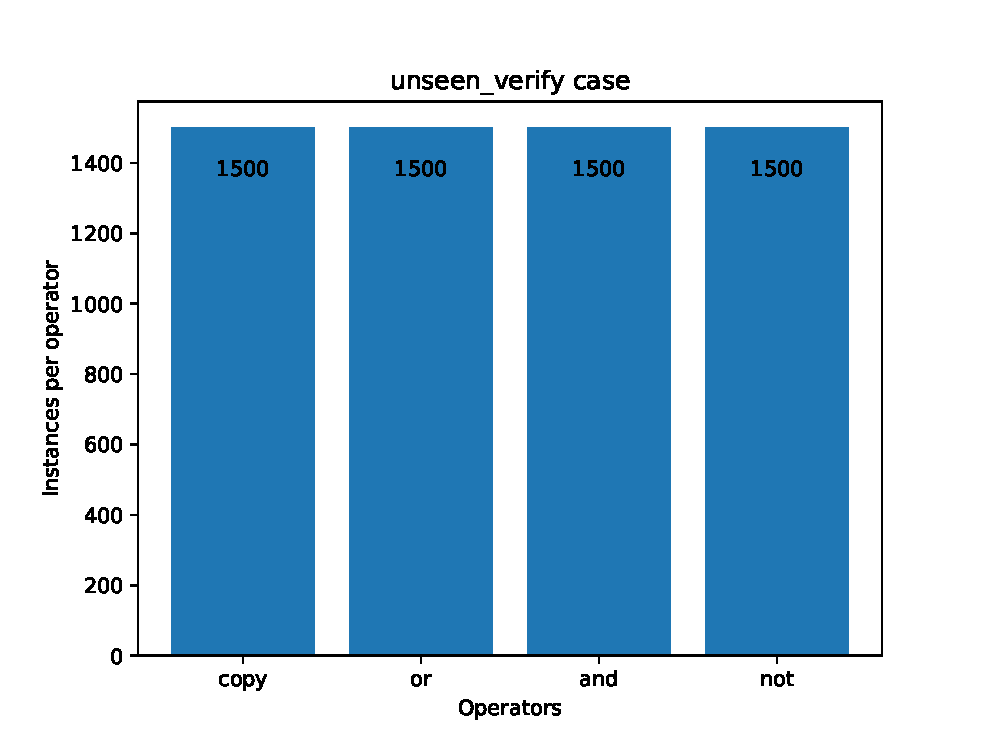
\includegraphics[width=0.95\linewidth]{./figs/micro/unseen_verify-eps}
		\fi
		\caption{Verification Task} 
		\label{un_ver} 
		\vspace{4ex}
	\end{subfigure}%% 
	\begin{subfigure}[b]{0.5\linewidth}
		\centering
		\ifpdf
		\includegraphics[width=0.95\linewidth]{./figs/micro/unseen_produce-pdf}
		\else
		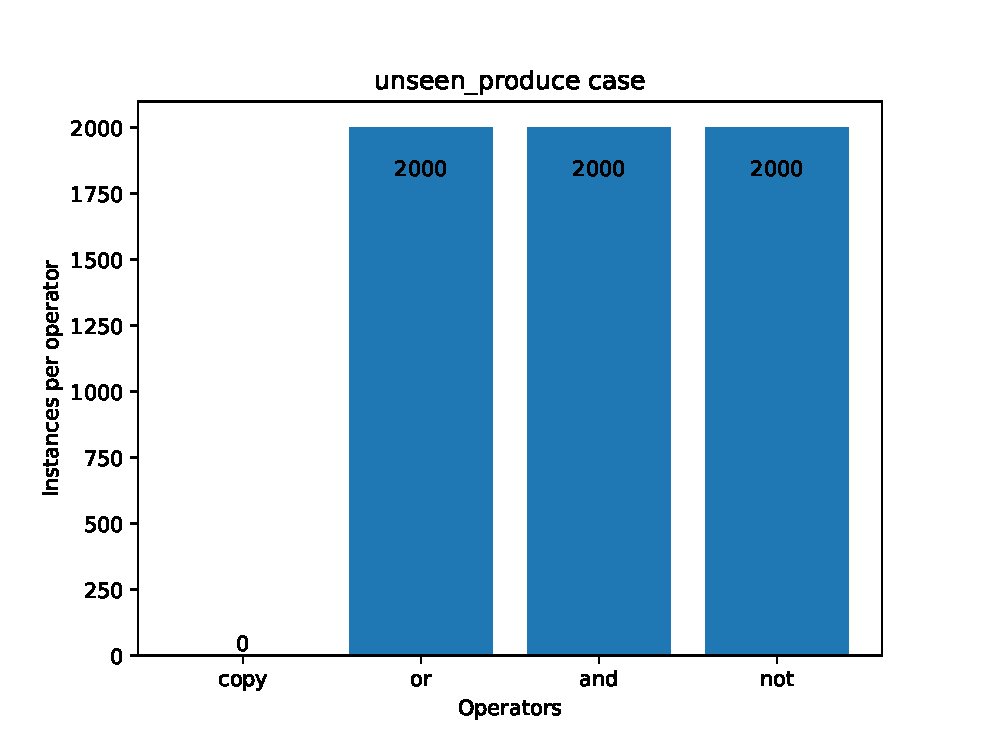
\includegraphics[width=0.95\linewidth]{./figs/micro/unseen_produce-eps}
		\fi 
		\caption{Production Task} 
		\label{un_prd} 
		\vspace{4ex}
	\end{subfigure}
	\caption{Micro Tasks - Unseen Data}
	\label{micro_test}
\end{figure}
    % Numerical Details and Algorithms
    \chapter{Experimental Setup}

Maths. Merge with previous chapter
    %Results and Discussions
    \begin{appendix}
	
\chapter{Algorithm for balancing lookup tables train set}\label{Chapter:results}

Since the dataset for the lookup tables is small -- even if length 2 compositions was created using tables \textit{t1} to \textit{t8}, there could only be 64 compositions which would bijectively map 8 3 bit inputs to 3 bit outputs thereby leading to a total of 512 samples only -- we try to ensure that the compositions present in the training data are uniformly distributed while simultaneously keeping the distribution of the output strings in the training data uniform as well. This ensures that the model doesn't get biased towards any particular composition or an output string. As has been explained in section \ref{lt:splits}, the heldout inputs set is created by randomly taking out 2 inputs for each of the 28 compositions in training. Therefore the resultant training set should have the following properties:
\begin{itemize}
	\item The total number of data points  $= 28*6 = 168$.
	\item There are 8 outputs. The total number of compositions that lead to a particular output $=168/8 = 21$.
\end{itemize}

.
\begin{algorithm}
	\caption{Create training with uniform distribution of both compositions and outputs}
	\begin{algorithmic}
		\STATE We start with 28 compositions with 8 inputs each.
		\STATE Create an empty dataframe of dimension (21,8) with the 8 output strings as it's columns.
		\STATE Create a dictionary Y with compositions as it's keys and values=0.
		\FOR {i in range [0, 21)}
		\FOR {output in dataframe column}
		\STATE Sample composition
		\IF{composition \textbf{not in} row[i] AND composition \textbf{not in} output column AND Y[composition] $<$ 21 }
		\STATE dataframe[i][output] = composition
		\STATE Y[composition] += 1
		\ELSE
		\STATE continue
		\ENDIF
		\ENDFOR
		\ENDFOR		
	\end{algorithmic}
\end{algorithm}

\end{appendix}
    %Conclusions anf Recommendations
    \chapter{Conclusions and Future Work}%

\section{Conclusions}
AG works
learning AG is hard



\section{Future Work}
Understander executor
Representation learning
Latent space
    % add more chapters here
    %\include{chap_theory}
    %
    %
    % Bibliography
    \bibliography{my_thesis}
    %\printbib{my_thesis}%
    %
    \appendix%
    %
    % and some appendices here
    %\include{app_math_model}%
    %
    %
\backmatter%
    %
    % index file here (not needed for a MSc thesis)
    %
\end{document}
